\chapter{Conclusiones}
\label{conclusiones}
%\cambiar{El gráfico comparativo que hace con Gukena y los otros sistemas electorales no va en las conclusiones. - HECHO: Se quitan los gráficos}
%\cambiar{Para el caso de colocar esta descripción antes, aclara que las mesas cierran en distintos horarios, pero puede ponerlas todas al mismo horario de cierre X, y en vez de nombrar las horas finales de carga de mesas, poner directamente “luego de 90 minutos estaban el 90\% de las mesas cargadas” por ejemplo.}
%\cambiar{Repite párrafos completos, ¿otra vez la figura 6.2 y figura 6.3? - HECHO: se quitan los gráficos}

El proceso electoral se divide en 5 etapas según el modelo de referencia \cite{conicet} (Figura \ref{graf:modeloReferencia})
\begin{figure}[h!]
    \begin{center}
        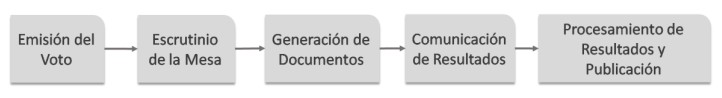
\includegraphics[width=\textwidth]{img/modeloReferencia.png}
    \end{center}
  \caption{Modelo de Referencia}
  \label{graf:modeloReferencia}
\end{figure}
\newline

Incluir tecnología sobre alguna de estas etapas consigue mejoras sobre el sistema electoral, por ejemplo acelerar la velocidad de procesamiento. Sin embargo, puede incluir problemas como  poner en riesgo la integridad y secreto del voto, principalmente cuando se incluye en la primera fase, Emisión del voto. En esta tesis se analizaron experiencias a nivel nacional e internacional, en muchos casos, luego de varios intentos los responsables de estas elecciones resolvieron no continuar con un sistema de voto electrónico. Un ejemplo de ello es Holanda, que luego de 9 años utilizando un sistema electrónico se demostraron las vulnerabilidades del sistema y el gobierno decidió volver al proceso electoral tradicional en papel. Un sistema electoral exitoso debe garantizar la confianza de toda persona involucrada, para ello, es necesario entender todo el proceso interno del sistema. Sin embargo, sólo un grupo reducido de personas relacionadas al área de sistemas computacionales comprenderán el funcionamiento de este proceso, aún así, no existe un método formal de validación que avale un sistema electrónico correcto. 

Luego de analizar en esta tesis las ventajas y desventajas de implementar tecnología en cada una de las etapas del proceso electoral, se expone el desarrollo e implementación del sistema Gukena. Este sistema mantiene las primeras 3 etapas (Emisión del voto, Escrutinio de la Mesa y Generación de Documentos) de forma tradicional en papel y manual. Gukena se integra en las etapas de Comunicación de Resultados, Procesamiento de Resultados y Publicación. La etapa de Comunicación de resultados es de manera descentralizada mediante un ``acta electrónica'' cargado por cada autoridad de mesa al finalizar el escrutinio. El sistema se encarga de procesar y publicar los resultados en tiempo real a medida que se van cargando los datos en este acta.

Gukena se incluye en las elecciones de la UNComa y consigue un cambio notable en este proceso, tanto a nivel de velocidad del escrutinio como de claridad y transparencia en los resultados finales. Previo a utilizar Gukena, estas elecciones eran administradas por una única persona. Todo este proceso abarcaba varios días debido a que se generaba un cuello de botella. Gukena logra distribuir la carga de trabajo a un grupo de personas, las autoridades de mesa y la Junta Electoral.

Por lo tanto, el proceso electoral de la UNComa con Gukena queda de la siguiente manera:
\begin{enumerate}
    \item Emisión del Voto: Tradicional en papel, colocando el sufragio en el sobre.
    \item Escrutinio de la Mesa: Tradicional escrutinio manual.
    \item Generación de Documentos: Tradicional utilizando el acta en papel.
    \item Comunicación de Resultados: Formulario de Gukena donde cada autoridad de mesa vuelca los datos del acta en papel.
    \item Procesamiento de Resultados y Publicación: Gukena realiza el procesamiento aplicando las fórmulas de ponderación y publica los resultados provisorios en tiempo real en su página web pública. Los datos recibidos de cada acta se validan por la Junta Electoral a través del sistema.
\end{enumerate}

En este documento se analizaron las experiencias de Gukena dentro del ámbito de la UNComa y se pudo observar que con una mínima incorporación de tecnología en el proceso electoral, sin invadir la etapa de Emisión del Voto, se lograron buenos resultados de velocidad del escrutinio sin afectar el secreto del voto y la auditabilidad del sistema.

Una de las ventajas adicionales que introdujo Gukena a la transparencia del proceso es la visualización de información histórica de elecciones a partir del 2015, información que no era pública y de fácil acceso previamente. Otra ventaja agregada es facilitar la comprensión de la fórmula del voto ponderado, explicada en conjunto con los resultados de cada elección, accesibles en cualquier momento desde cualquier dispositivo con acceso a Internet a través de la página web. Gukena fue expuesto en el artículo presentado en la JAIIO describiendo lo planteado en este capítulo \cite{articuloGukena}.

Además, en este trabajo se agregó la evaluación del escrutinio de las elecciones en la provincia de Córdoba, Rio Negro y Neuquén realizadas en el año 2019, junto con las experiencias de Gukena en el año 2018. Cada una de estas elecciones aplicó distintas técnicas de conteo durante el proceso electoral, la velocidad de las elecciones en Córdoba y Río Negro es constante durante todo el escrutinio. Por otro lado, en la provincia de Neuquén y con Gukena se logró en poco tiempo conseguir la mayoría de las mesas escrutadas disponibles en el sistema, satisface el objetivo de reducir los tiempos con respecto al sistema tradicional. Sin embargo, el horario de finalización del escrutinio no varía mucho en cada elección, por lo tanto, aplicar tecnología en cualquier etapa del proceso electoral no genera un impacto notable en el horario de publicación de resultados.

Otra característica, en las elecciones de Neuquén se deben capacitar los técnicos (mínimo uno por escuela), las autoridades de mesa y cada votante. En cambio, Gukena sólo necesita la capacitación de una persona por mesa, cada autoridad de mesa recibe un instructivo en papel incluido en el kit de la urna. Esta ventaja de Gukena reduce notablemente el presupuesto en capacitación.

Además del desarrollo e implementación de Gukena, como aporte a esta tesis, se presenta una encuesta realizada a los votantes de Neuquén Capital con respecto al sistema BUE. Más de la mitad de los encuestados no conocía la existencia del lector de chip, por lo tanto, se podría concluir que si existieron errores de escritura no fueron detectados. A partir de este análisis se sugirió a nivel provincial un cambio de protocolo en las elecciones electrónicas en la Junta Electoral Provincial. Este cambio consta de una validación de manera aleatoria de las máquinas BUE durante el acto electoral, agregando una verificación más dentro de este proceso. La validación consta de imprimir una boleta y verificarlo con el lector de la máquina corroborando su correcta escritura del chip. Esta sugerencia fue tomada en cuenta y es aplicada a partir del 2019 en las elecciones dentro de la provincia del Neuquén.


\section{Trabajos Futuros}

Como trabajo sugerido a futuro en Gukena está asociado a la posibilidad de incluir la Boleta Única en papel dentro del sistema electoral de la UNComa. Esta boleta consiste en un solo papel por categoría a votar, por ejemplo para las elecciones en UNComa del año 2018, descripto en la Sección \ref{gukena2018}, cada votante va a disponer de 4 boletas únicas en papel, uno por cada categoría. Esto reduce notablemente la gran cantidad de papeles y en presupuesto general, actualmente se dispone de un papel por cada lista y por cada categoría. Las ventajas de la Boleta Única en Papel y un ejemplo de ésta se describe en el Anexo \ref{BU}. El posible cambio a nivel de proceso electoral impacta en el formulario de carga de Gukena, obligando a incorporar nuevas validaciones o cambios, como por ejemplo, la cantidad de votantes puede diferir por categoría, validación no contemplada actualmente. Esto aplica a la propiedad de calidad, descripta en la sección \ref{propiedadesCalidad}, de cumplir con las normativas vigentes del proceso electoral, Gukena debe adaptarse a cualquier cambio sobre el proceso electoral en UNComa. 
%\cambiar{¿Por qué se coloca un anexo de la boleta única en papel? y Gukena?}

Un cambio pendiente en Gukena a nivel desarrollo, es incluir las actas escaneadas o imagen dentro del formulario de carga, para que estén disponibles en la página web. Actualmente, los usuarios (Autoridades de Mesa más lejanos del centro de cómputos) deben enviar la imagen del acta por algún medio que logre llegar a la Junta Electoral para su validación. Como no existe una única vía de comunicación, se debe estar atento en reconocer el medio utilizado por cada autoridad de mesa: fax, mensaje privado, email o presencial. Con una carga de archivos de imágenes dentro de los datos en el formulario de carga, se generaría un único medio de fácil acceso por la Junta Electoral y la Secretaria para su validación.
Agregar este cambio no reemplazaría el envío al centro de cómputos del acta en papel y la urna con los votos, como registro físico auditable de la elección. 
